% Chapter Template

\chapter{Results and Discussions} % Main chapter title

\label{ChapterX} % Change X to a consecutive number; for referencing this chapter elsewhere, use \ref{ChapterX}

\lhead{Chapter X. \emph{Chapter Title Here}} % Change X to a consecutive number; this is for the header on each page - perhaps a shortened title

%----------------------------------------------------------------------------------------
%	SECTION 1
%----------------------------------------------------------------------------------------

The application - "A Fun virtual Cam" was made, which can understand the sentiment of the person and change the video background accordingly to create a better experience, while delivering an average frame rate of 38fps on a 1080p camera.

\section{Outputs}
\begin{figure}[H]
\centering
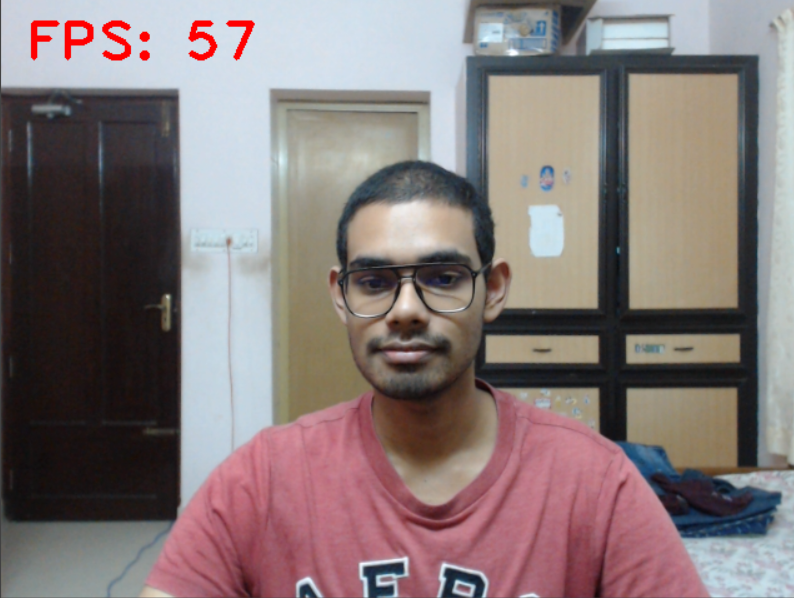
\includegraphics[width = .8\textwidth]{Images/DesProOutput1}
\caption{Frame without background change}
\label{List of organizations}
\end{figure}

\begin{figure}[H]
\centering
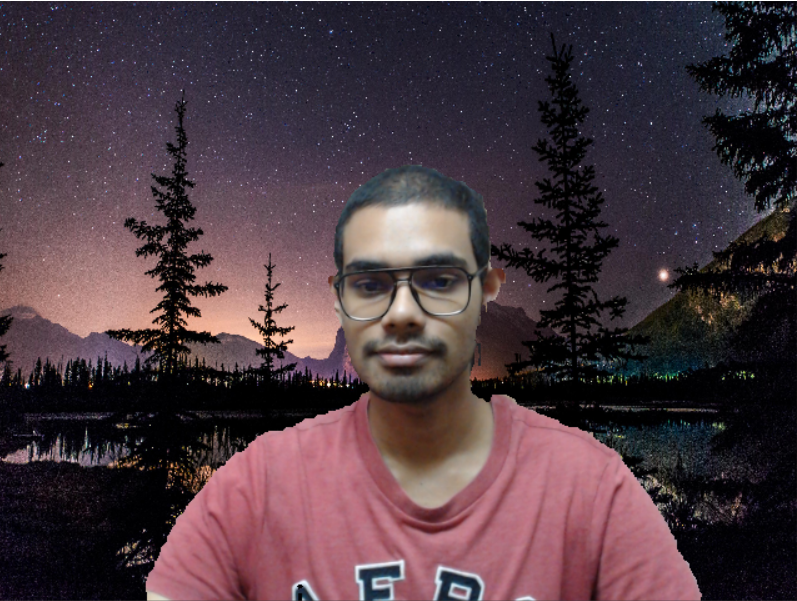
\includegraphics[width = .8\textwidth]{Images/DesProOutput2}
\caption{Frames with background change}
\label{List of organizations}
\end{figure}

\begin{figure}[H]
\centering
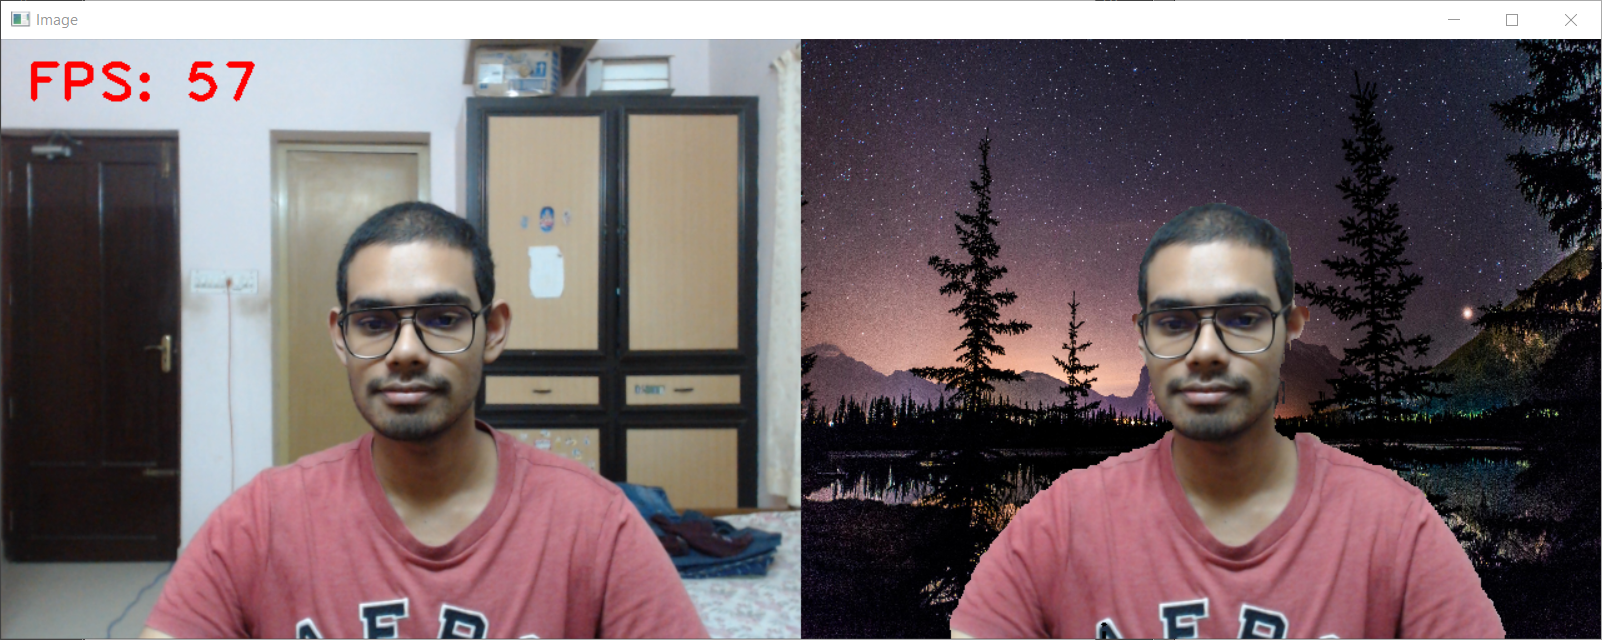
\includegraphics[width = .8\textwidth]{Images/DesProOutput}
\caption{Frames with and without background}
\label{List of organizations}
\end{figure}

\begin{figure}[H]
\centering
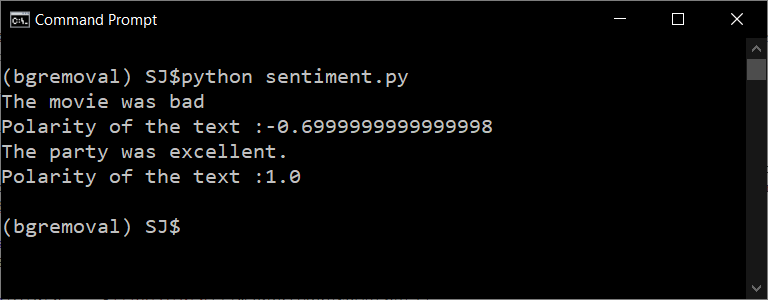
\includegraphics[width = .8\textwidth]{Images/Polarity}
\caption{Output - Polarity calculation}
\label{List of organizations}
\end{figure}

